\documentclass[10pt,a4paper]{article}
\usepackage[utf8]{inputenc}
\usepackage[T1]{fontenc}
\usepackage{lmodern}
\usepackage[margin=20mm]{geometry}
\usepackage{graphicx}
\usepackage{amsmath,amssymb}
\usepackage{booktabs,longtable,array}
\usepackage{caption}
\usepackage{xcolor}
\usepackage{hyperref}
\usepackage{microtype}
\usepackage{fancyhdr}
\usepackage{float}
\hypersetup{colorlinks=true,linkcolor=blue,urlcolor=blue}
\pagestyle{fancy}
\fancyhf{}
\fancyhead[R]{\small EE3005 | Biomedical System Design Capsule-S1}
\fancyfoot[R]{\small Burak Bekir Çakırer / 2211011008 / \thepage}
\setlength{\headheight}{14pt}
\begin{document}
\begin{center}
{\LARGE\bfseries BIOMEDICAL SYSTEM DESIGN CAPSULE-S1}\\[7pt]
{\large EE3005 -- Assignment 2: Image Processing}\\[5pt]
{\large Image Enhancement, Filtering and Edge Detection}\\[13pt]
{\bfseries Burak Bekir Çakırer}\\
Student ID: 2211011008\\
Course: EE3005 -- BIOMEDICAL SYSTEM DESIGN CAPSULE-S1\\[8pt]
\textbf{GitHub repository (active after publication):}\\
\url{https://github.com/burakcakirer/ee3005-image-processing-assignment-2}
\end{center}
\smallskip
\noindent\textit{Technical note: Figures and tables are generated by the executed Python reference. MATLAB source is supplied and requires separate execution. Not for clinical decision making.}
\tableofcontents
\newpage
\section{Abstract}
This study evaluates eight complementary biomedical image processing tasks: local contrast enhancement, correlation and convolution, boundary padding, separable filtering, linear and nonlinear denoising, sharpening, gradient/second-order edge detection, and an integrated workflow. The experiments use two images from the supplied course archive and fixed synthetic noise inputs. Visual comparisons are supported by explicit calculations, PSNR, and documented parameter selections. The source implementations are maintained as independent project files and are intentionally not printed in this report.

\section{Experimental setup and reproducibility}
This report covers all eight tasks in EE3005 Biomedical System Design Capsule-S1, Assignment 2. The radiograph-like chest image (image3.jpg, 800 x 752 pixels) is used for local contrast, border padding, and the integrated processing pipeline. The axial brain MRI example (image2.jpg, 617 x 617 pixels) is used for filtering, sharpening, and derivative operators. These images were supplied in the course assignment archive. Their external creators, licenses, acquisition parameters, and clinical context were not provided; therefore, no diagnostic claims are made. A visible Kenhub logo/watermark remains in the supplied MRI image.

All experiments operate on explicitly saved 8-bit grayscale PNG inputs scaled to [0,1]. MATLAB source is supplied in MATLAB/run\_assignment2.m; the experiments load the same fixed source and noise PNG files. A fully executed Python reference implementation generates the figures and numerical results in this report (NumPy/SciPy/scikit-image/OpenCV). The MATLAB implementation was prepared but not executed in this environment; library-specific AHE/CLAHE interpolation, boundary conventions, and rounding can change individual results. For an exact MATLAB-origin report, rerun the MATLAB script and refresh the tables and figures.

Python reference settings: random generator seed 3005; Gaussian noise standard deviation 0.06 (normalized intensity); combined salt-and-pepper noise density 0.08 (equal salt and pepper fractions); independent salt-only and pepper-only densities 0.08. Prepared noisy realizations are frozen as PNG files so that method comparisons use identical contaminated pixels. Unless otherwise indicated, filtering uses mirrored-edge/half-sample symmetric extension, intensities are clipped to [0,1], and PSNR is computed relative to the corresponding clean input.

\section{Task 1 - Adaptive histogram equalization and CLAHE}
The chest radiograph contains dark peripheral areas and relatively low-separation gray tones around internal thoracic structures; a single global gray-level mapping cannot independently tune each locality. Figure 1 compares the input with global histogram equalization (HE), a virtually unlimited local AHE configuration (8 x 8 tiles, clip limit 1.0), and two contrast-limited configurations (8 x 8, clip 0.01; 16 x 16, clip 0.03). Histogram bin count is 256 for processing; the plotted histograms use 64 bins for readability.

\begin{figure}[!htbp]
\centering
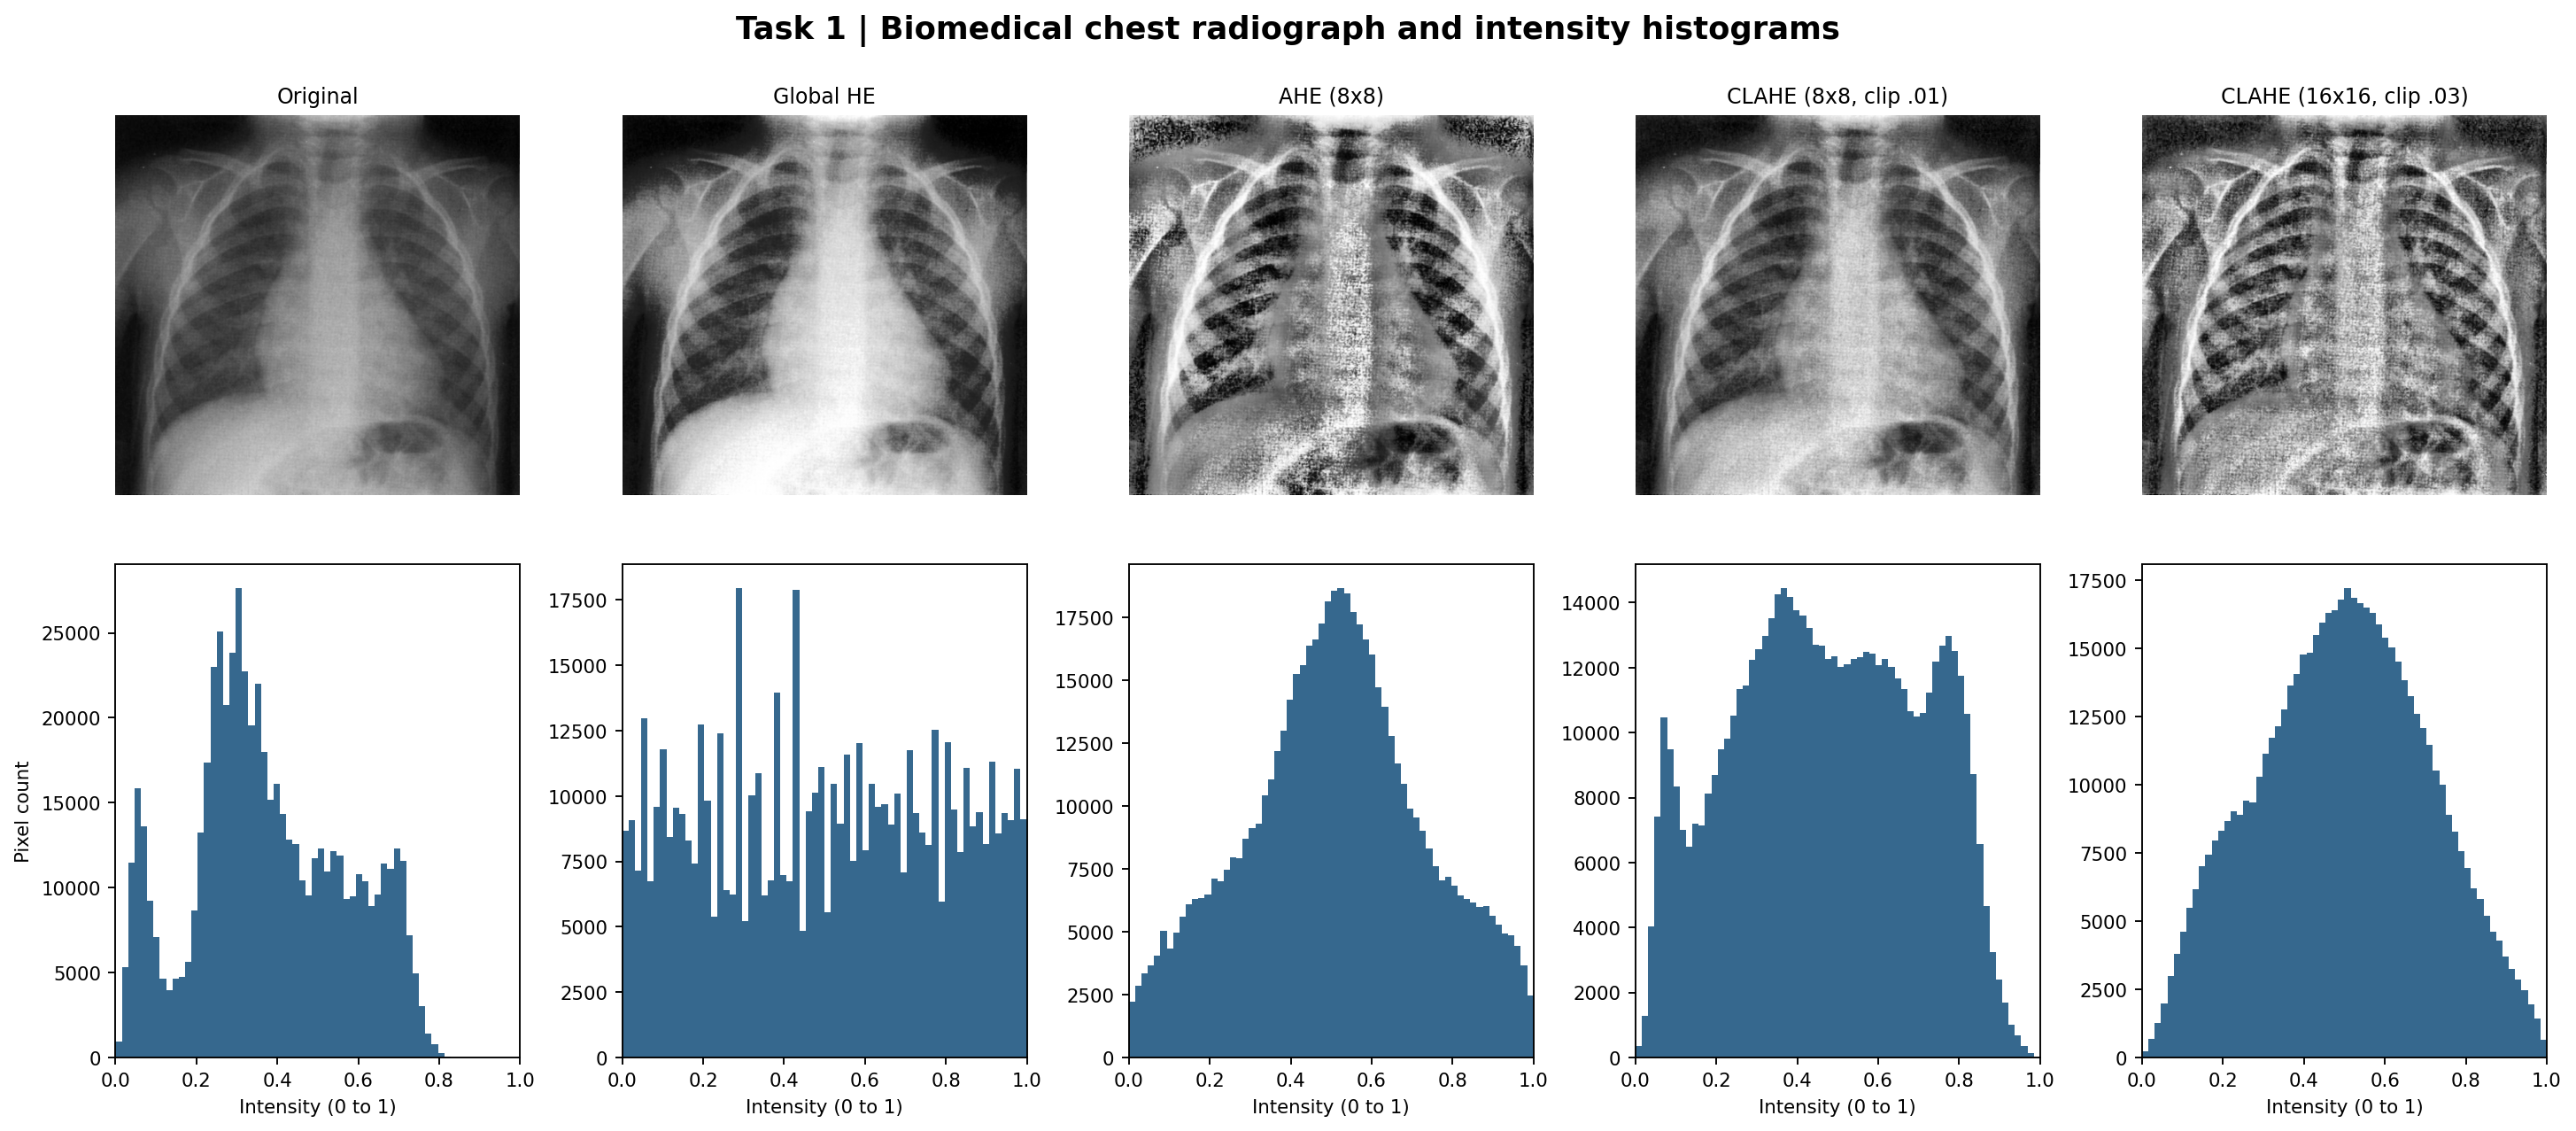
\includegraphics[width=\linewidth,height=0.72\textheight,keepaspectratio]{Figures/F01_contrast_histograms.png}
\caption{Input, global HE, AHE, and two CLAHE configurations with corresponding intensity histograms.}
\end{figure}
\begin{longtable}{|p{50.0mm}|p{50.0mm}|p{50.0mm}|}
\caption{Measured intensity standard deviation (normalized units)}\\
\hline
\textbf{Method} & \textbf{Whole image} & \textbf{Central ROI}\\ \hline
\endfirsthead
\hline
\textbf{Method} & \textbf{Whole image} & \textbf{Central ROI}\\ \hline
\endhead
Original & 0.1908 & 0.1658\\ \hline
Global HE & 0.2883 & 0.2670\\ \hline
AHE 8x8 & 0.2222 & 0.2054\\ \hline
CLAHE 8x8 / .01 & 0.2294 & 0.2254\\ \hline
CLAHE 16x16 / .03 & 0.2090 & 0.1924\\ \hline
\end{longtable}
For the defined central ROI (rows 190-469, columns 210-509 in zero-based Python indexing), local variation rises from 0.166 to 0.225 under moderate CLAHE. Global HE spreads the overall histogram most strongly (0.288 versus 0.191 originally) but also changes the dark background substantially. AHE treats each region locally, bringing out soft tissue and rib boundaries but also enhancing grain; CLAHE limits histogram-bin accumulation before redistribution to suppress that tendency. Reducing the tile size to 16 x 16 tiles while increasing clip limit to .03 changes enhancement spatially; it does not guarantee a higher global standard deviation.

On visual comparison, CLAHE 8 x 8 / 0.01 is a cautious choice because anatomical contours become easier to distinguish without the most aggressive enhancement of background texture. Increased histogram spread is not, by itself, evidence of increased medical usefulness; subjective visibility and preservation of noise and artifacts must also be considered. [1, 2]

\section{Task 2 - Correlation, convolution, and border effects}
A 3 x 3 kernel defines how neighboring intensities contribute to each filtered pixel. The assignment specifies the asymmetric horizontal derivative kernel and a 5 x 5 image matrix. At image center (row 3, column 3, one-based indexing), the extracted neighborhood is:

\[ P=\begin{bmatrix}25&35&45\\30&40&50\\35&45&55\end{bmatrix},\quad K=\begin{bmatrix}1&0&-1\\2&0&-2\\1&0&-1\end{bmatrix} \]
Correlation uses K unchanged. The nine elementwise products are [25, 0, -45; 60, 0, -100; 35, 0, -55]. Their sum is (25 - 45) + (60 - 100) + (35 - 55) = -20 - 40 - 20 = -80.

Convolution rotates K by 180 degrees: K\_flip = [-1, 0, 1; -2, 0, 2; -1, 0, 1]. The products are [-25, 0, 45; -60, 0, 100; -35, 0, 55]. The sum is (-25 + 45) + (-60 + 100) + (-35 + 55) = 20 + 40 + 20 = +80. The sign reversal occurs because K is antisymmetric under 180-degree rotation. These calculations are also independently checked by the program and saved to task02\_manual\_calculations.txt.

Border handling is evaluated on a fixed 510 x 455 chest crop using a normalized 3 x 3 arithmetic mean kernel. Zero adds artificial black samples; replication repeats the nearest available boundary pixel; mirror reflects adjacent interior pixels without repeating the edge pixel; circular wraps the opposite side of the crop into the kernel.

\begin{figure}[!htbp]
\centering
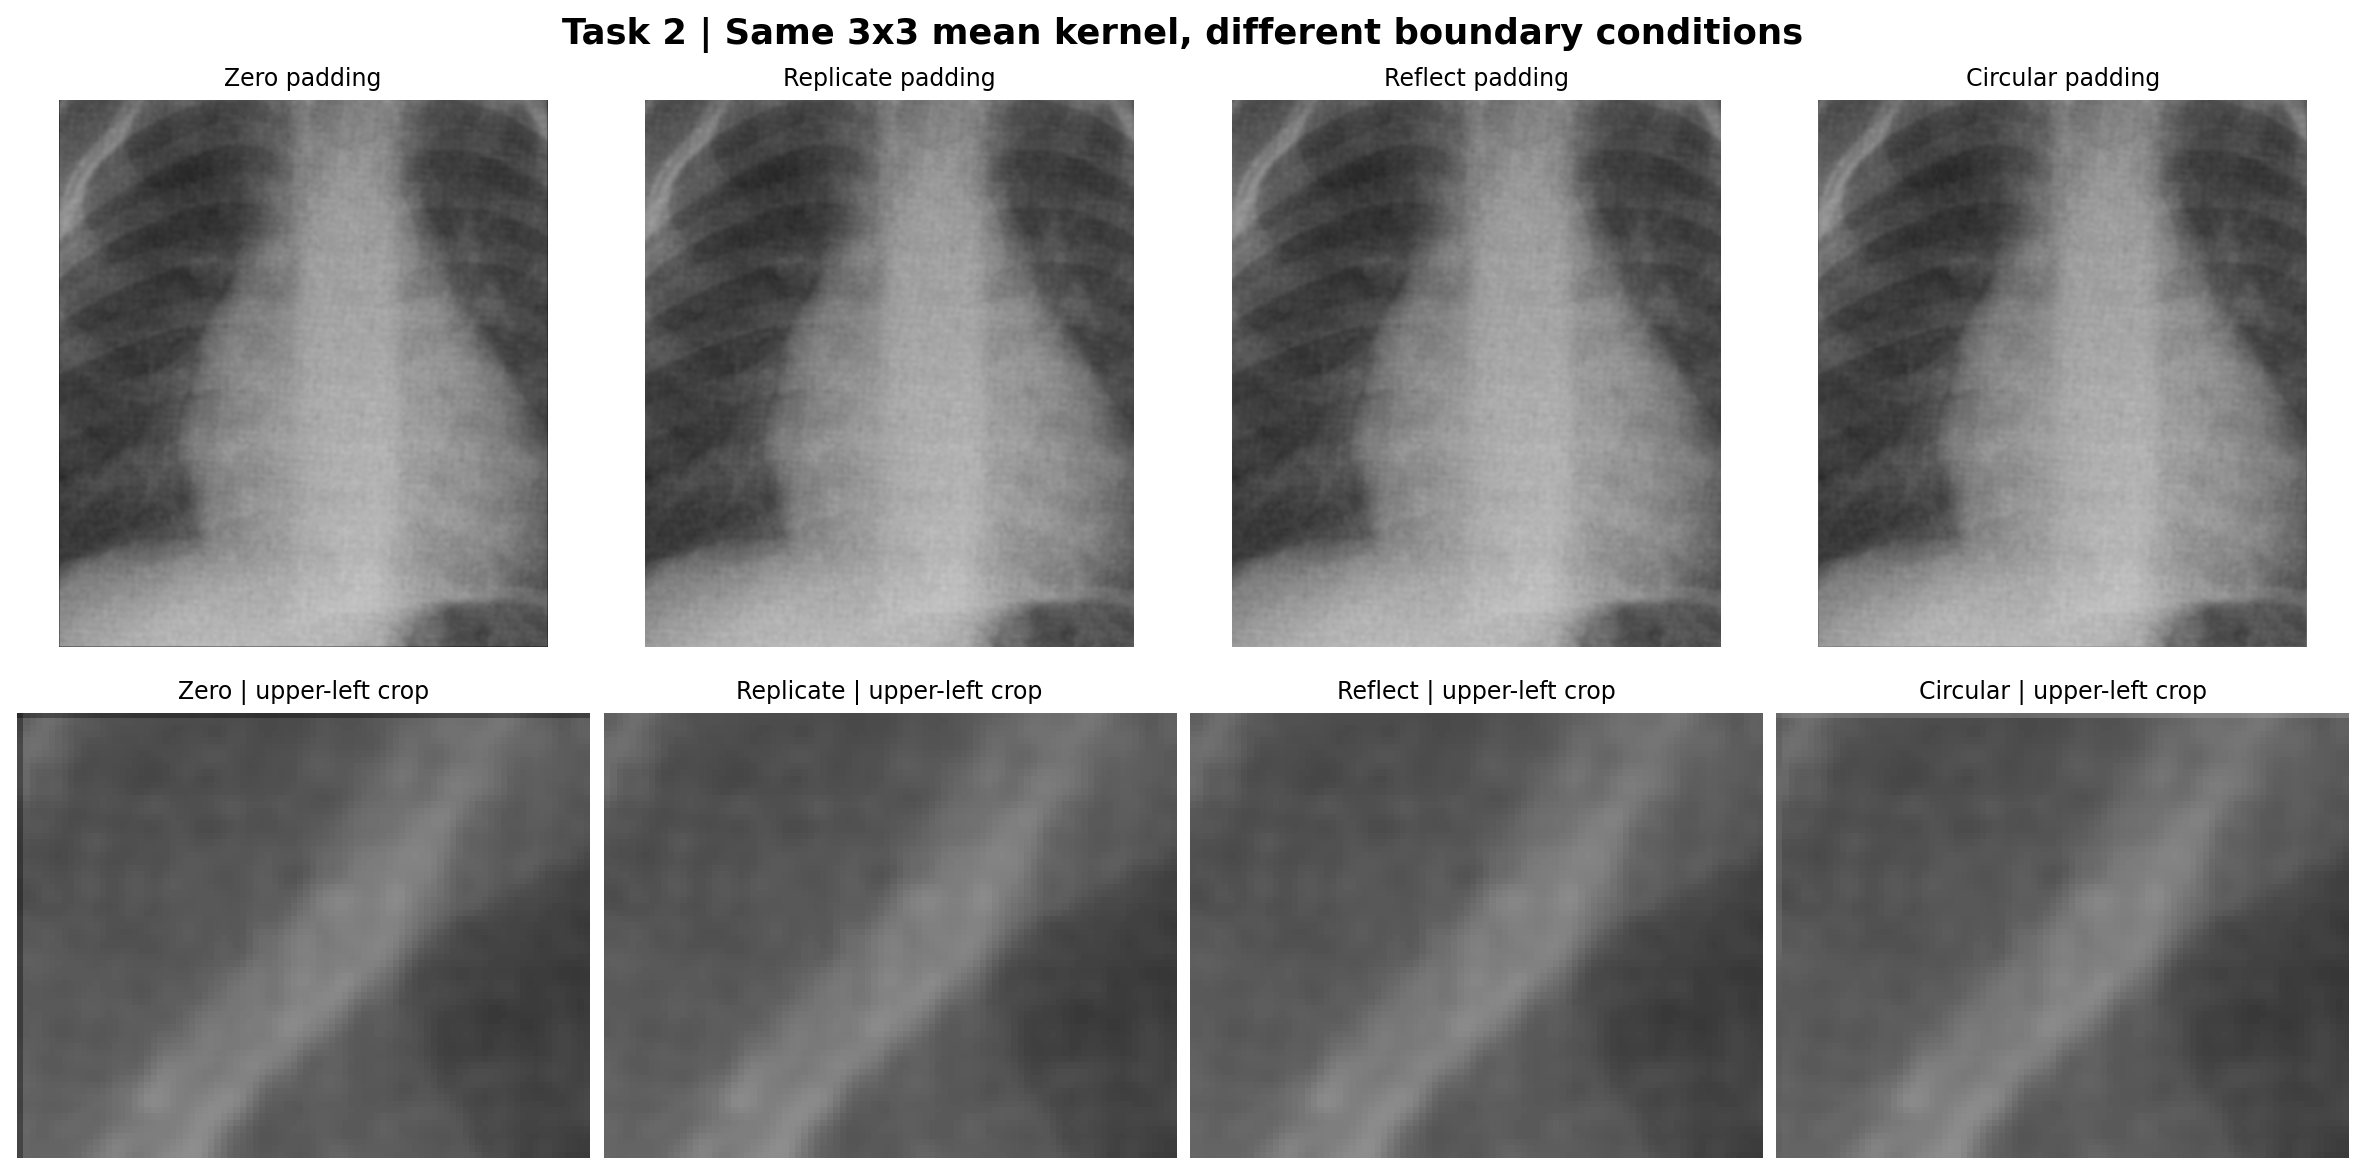
\includegraphics[width=\linewidth,height=0.72\textheight,keepaspectratio]{Figures/F02_padding_comparison.png}
\caption{Four padding strategies; bottom row magnifies their upper-left output regions.}
\end{figure}
\begin{longtable}{|p{75.0mm}|p{75.0mm}|}
\caption{Mean absolute difference from mirror on one-pixel outer border}\\
\hline
\textbf{Padding rule} & \textbf{Boundary MAE}\\ \hline
\endfirsthead
\hline
\textbf{Padding rule} & \textbf{Boundary MAE}\\ \hline
\endhead
Zero & 0.13888\\ \hline
Replicate & 0.00239\\ \hline
Reflect & 0.00000\\ \hline
Circular & 0.05738\\ \hline
\end{longtable}
Relative to mirror, zero padding has a substantial one-pixel-border deviation (0.1389), while replication produces 0.0024; circular wrapping gives 0.0574. The inner image agrees across methods, because the 3 x 3 footprint remains within the image there. Mirror is a reasonable default for this non-periodic crop, but replication can be preferable for genuinely constant edge regions, and circular padding is appropriate for periodic measurements or tiled textures. No padding scheme is universally optimal. [1, 3]

\section{Task 3 - Separable filtering and computational efficiency}
\[ K=\frac1{16}\begin{bmatrix}1&2&1\\2&4&2\\1&2&1\end{bmatrix}=\left(\frac14\begin{bmatrix}1\\2\\1\end{bmatrix}\right)\left(\frac14\begin{bmatrix}1&2&1\end{bmatrix}\right) \]
Multiplying the column and row vectors yields the exact original 3 x 3 Gaussian kernel. The direct method applies all nine coefficients at each output pixel, while the separable method performs three horizontal and three vertical multiplications per pixel. This reduces the arithmetic work from K\textasciicircum{}2 to 2K (9 versus 6 multiplications per interior pixel, approximately 33\% fewer); memory traffic and boundary overhead may influence real execution time.

\begin{figure}[!htbp]
\centering
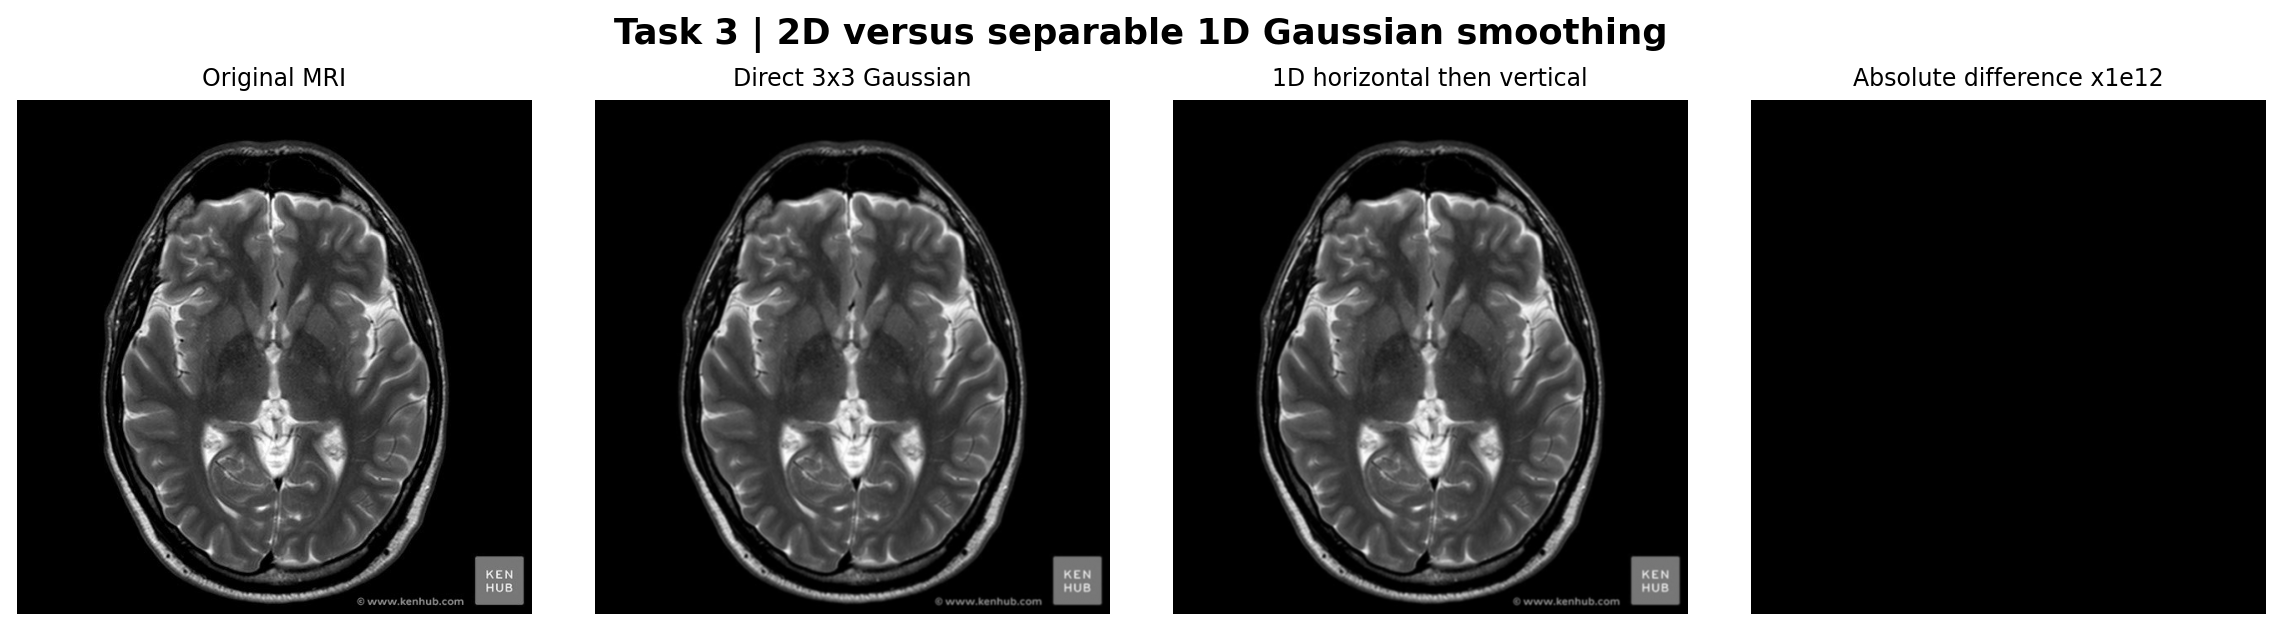
\includegraphics[width=\linewidth,height=0.72\textheight,keepaspectratio]{Figures/F03_separable_gaussian.png}
\caption{Direct 2D Gaussian versus successive horizontal/vertical 1D filtering on the MRI input.}
\end{figure}
The observed maximum absolute difference is 3.331e-16. This is floating-point rounding, not a visibly meaningful structural change. Using different border policies, clipping intermediate values, integer image types, or non-identical kernels would cause larger disagreements. Both implementations use the same mirrored boundary policy and double-precision operations. [1, 3]

\section{Task 4 - Linear filtering for noise reduction}
\[ \mathrm{PSNR}=10\log_{10}\left(\frac1{\mathrm{MSE}}\right),\quad\mathrm{MSE}=\frac1{MN}\sum_{x,y}(f(x,y)-g(x,y))^2 \]
The same clean MRI is retained throughout all comparisons. Gaussian noise causes distributed small-amplitude fluctuations (standard deviation 0.06), whereas 8\% impulse noise replaces selected pixels with full black or white. Mean filters of size 3 x 3 and 5 x 5 and Gaussian filters of size 3 x 3 (sigma 0.8) and 7 x 7 (sigma 1.4) are applied to both noisy inputs. Intensities are compared on a common 0 to 1 range.

\begin{figure}[!htbp]
\centering
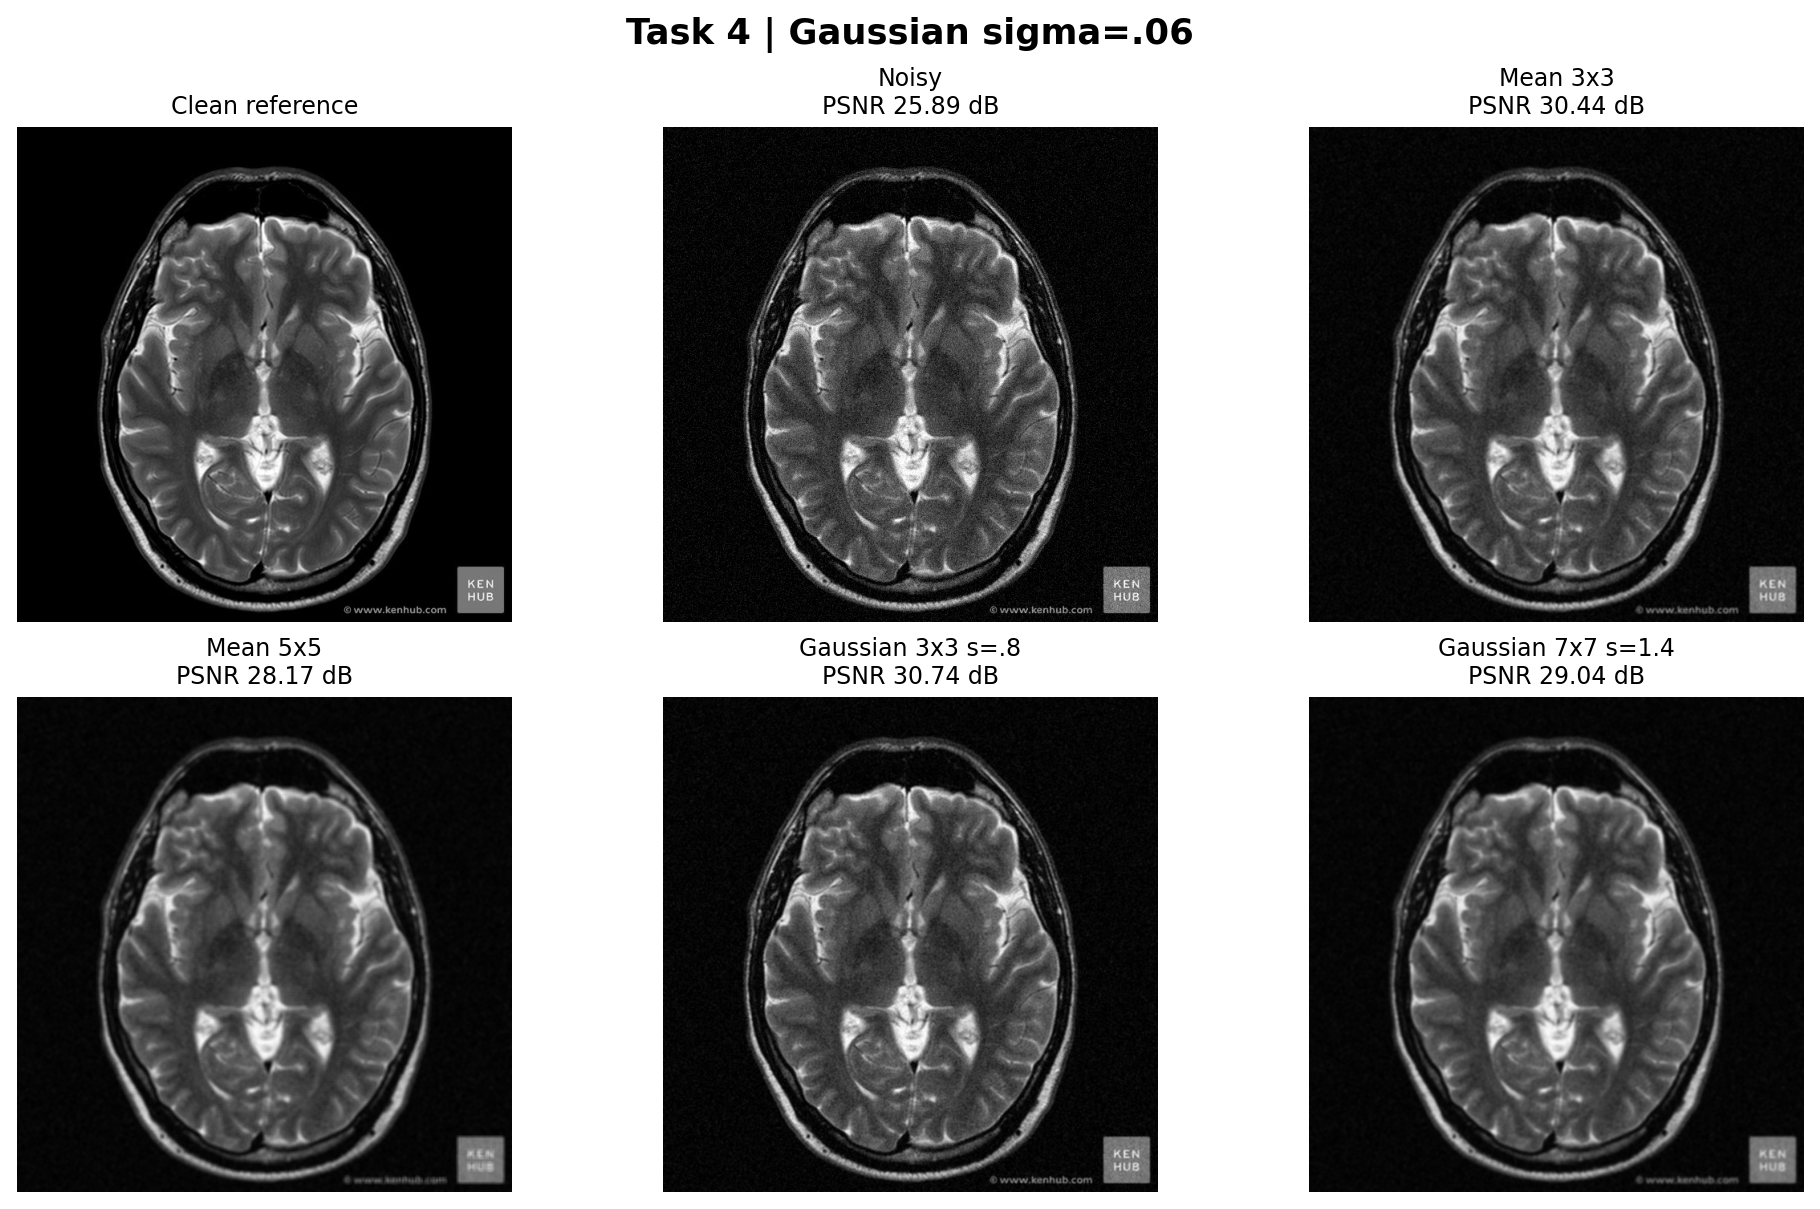
\includegraphics[width=\linewidth,height=0.72\textheight,keepaspectratio]{Figures/F04_gaussian_filtering.png}
\caption{Gaussian-noise case: identical corrupted input, then four linear smoothing alternatives.}
\end{figure}
\begin{figure}[!htbp]
\centering
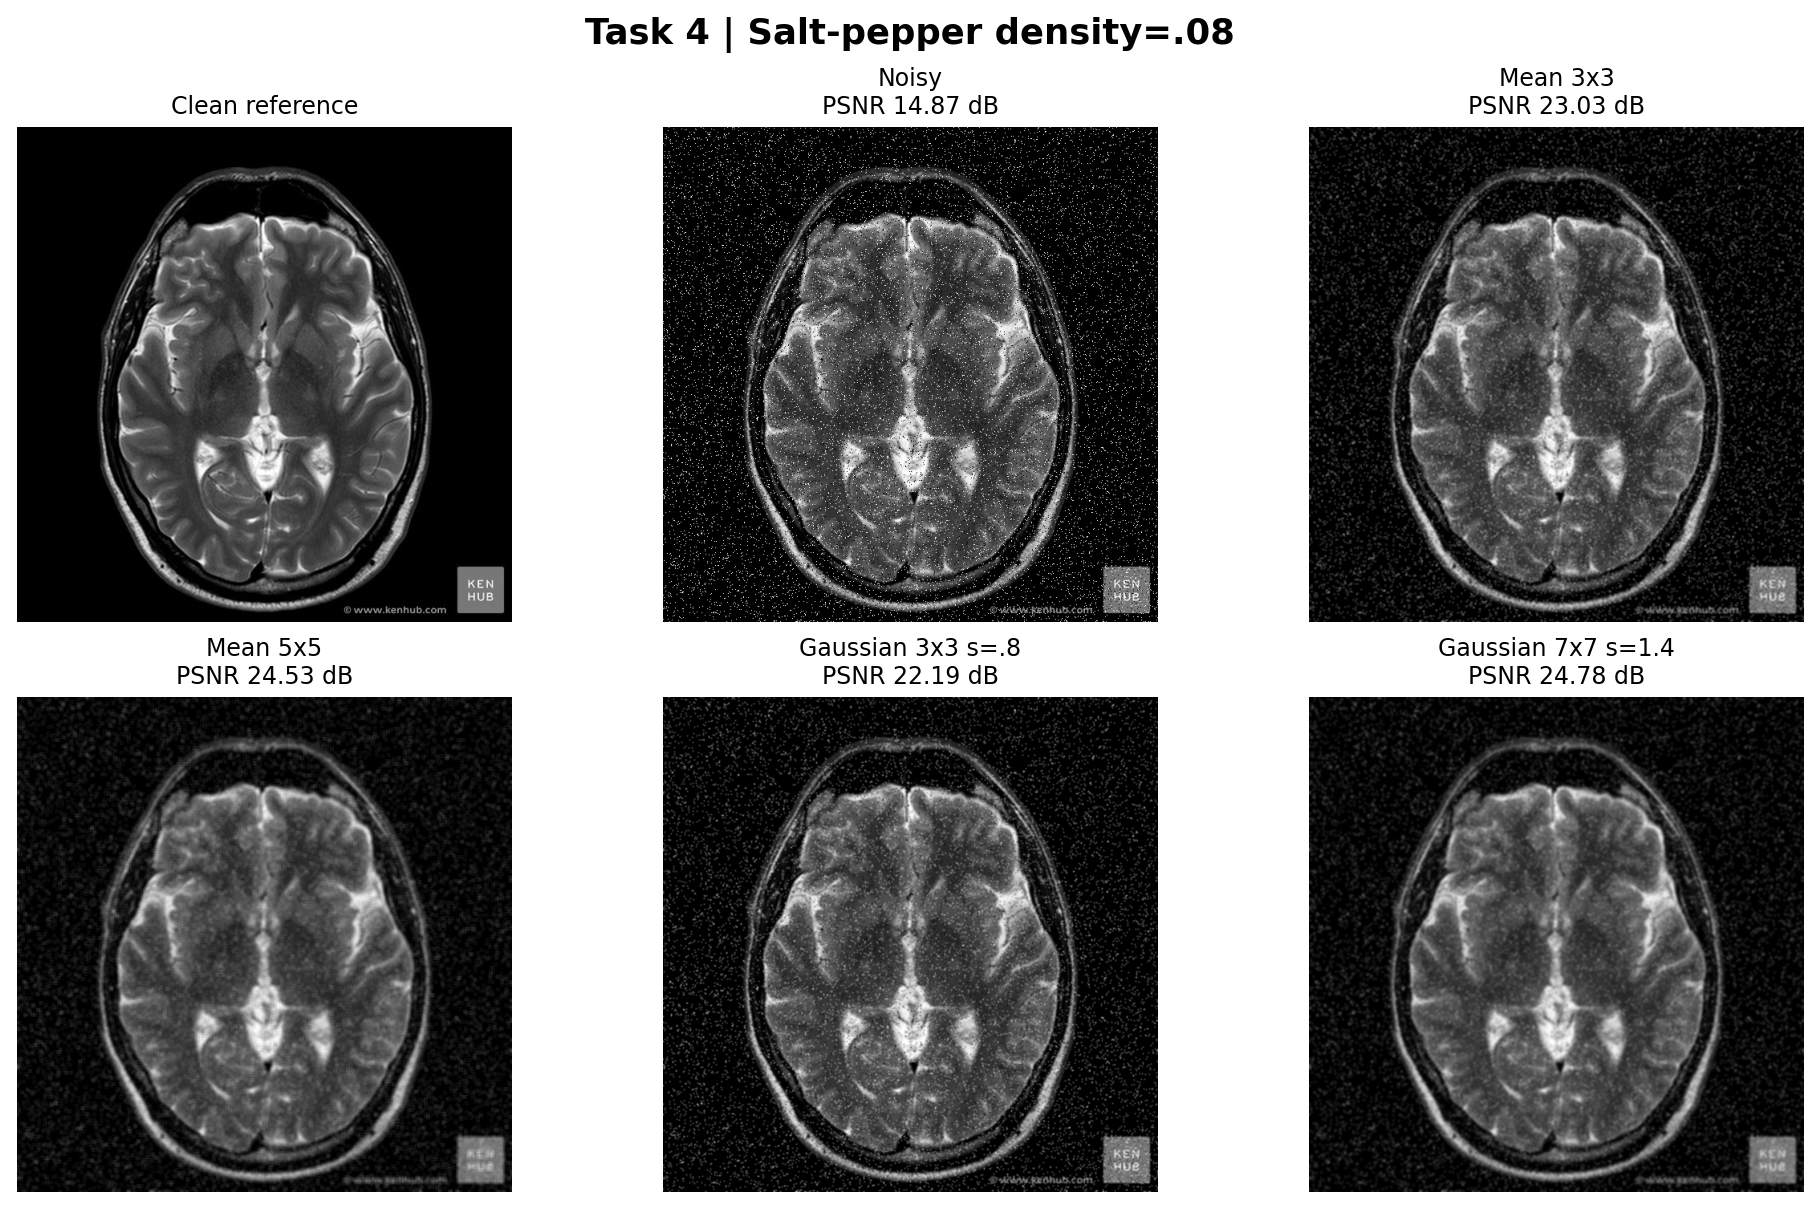
\includegraphics[width=\linewidth,height=0.72\textheight,keepaspectratio]{Figures/F04_impulse_filtering.png}
\caption{Salt-and-pepper case: same linear filters and their reconstruction PSNR values.}
\end{figure}
\begin{longtable}{|p{50.0mm}|p{50.0mm}|p{50.0mm}|}
\caption{Linear filtering PSNR (dB), higher is better}\\
\hline
\textbf{Noise model} & \textbf{Method} & \textbf{PSNR}\\ \hline
\endfirsthead
\hline
\textbf{Noise model} & \textbf{Method} & \textbf{PSNR}\\ \hline
\endhead
Gaussian & Noisy & 25.89\\ \hline
Gaussian & Mean 3x3 & 30.44\\ \hline
Gaussian & Mean 5x5 & 28.17\\ \hline
Gaussian & Gaussian 3x3 s=.8 & 30.74\\ \hline
Gaussian & Gaussian 7x7 s=1.4 & 29.04\\ \hline
Salt-pepper & Noisy & 14.87\\ \hline
Salt-pepper & Mean 3x3 & 23.03\\ \hline
Salt-pepper & Mean 5x5 & 24.53\\ \hline
Salt-pepper & Gaussian 3x3 s=.8 & 22.19\\ \hline
Salt-pepper & Gaussian 7x7 s=1.4 & 24.78\\ \hline
\end{longtable}
For the Gaussian realization, the best tested linear option is Gaussian 3x3 s=.8 with 30.74 dB, up from 25.89 dB in the noisy input. For the impulse realization, Gaussian 7x7 s=1.4 reaches 24.78 dB, although its impulse rejection is still much poorer than the 3 x 3 median result in Task 5. Increasing the smoothing footprint suppresses isolated fluctuations but also merges fine gyri/sulci outlines and other narrow transitions. PSNR indicates pixel-wise fidelity to this reference, not an independently established measure of diagnostic utility. [1, 3]

\section{Task 5 - Median and nonlinear mean filtering}
For impulse corruption, a median selects the middle-ranked sample rather than averaging extreme black or white outliers. A small 3 x 3 median therefore often restores local backgrounds and edges without pulling each neighbor toward a single corrupted value. The 5 x 5 neighborhood is more aggressive and may remove legitimately narrow structures.

\begin{figure}[!htbp]
\centering
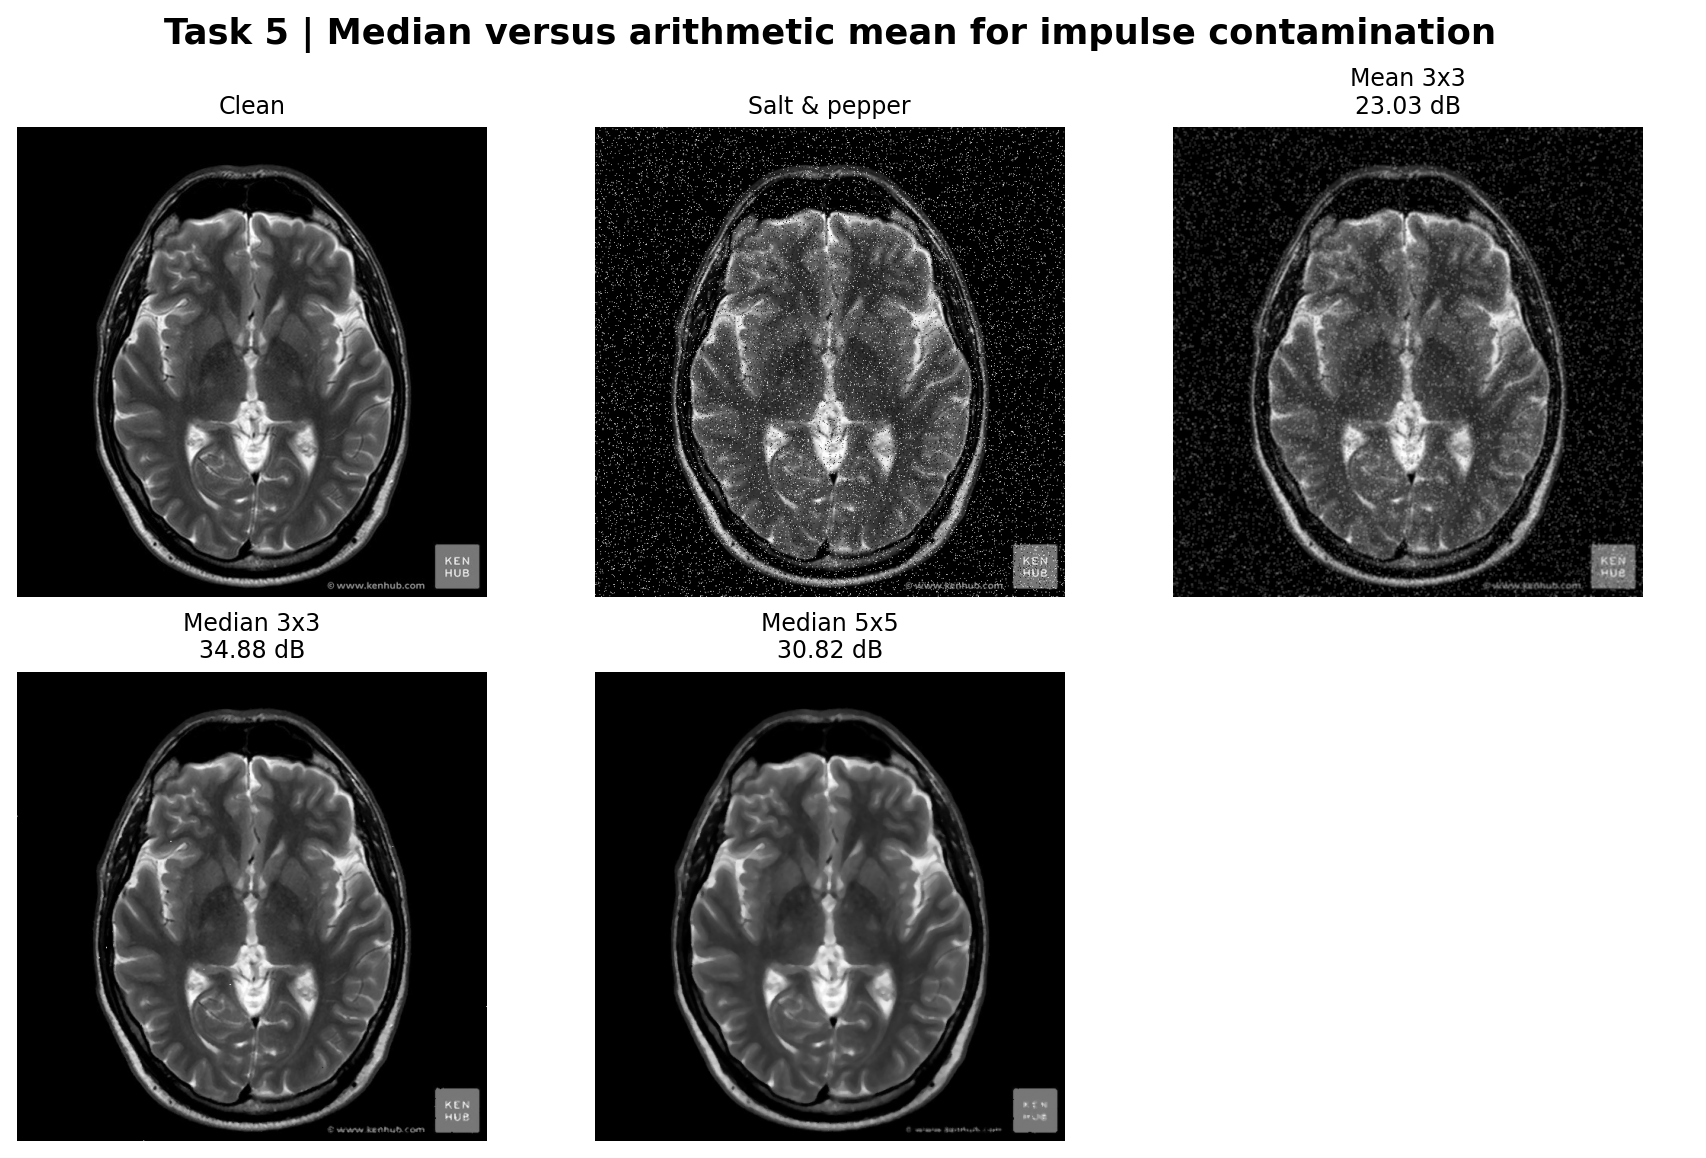
\includegraphics[width=\linewidth,height=0.72\textheight,keepaspectratio]{Figures/F05_median_impulse.png}
\caption{Direct comparison of noisy input, arithmetic mean, and 3 x 3 / 5 x 5 median filters.}
\end{figure}
\[ G=\left(\prod_{i=1}^{n}x_i\right)^{1/n},\quad H=\frac{n}{\sum_i1/x_i},\quad C_Q=\frac{\sum_i x_i^{Q+1}}{\sum_i x_i^{Q}} \]
The geometric mean is computed as exp(mean(log(max(x, 1/255)))) and the harmonic mean as 1 / mean(1/max(x, 1/255)), avoiding a logarithm or division by zero. This numerical intensity floor is itself a modeling choice and can alter deep-black pixels. The contra-harmonic filter uses Q=+1.5 or -1.5; when Q is negative, the same 1/255 floor prevents division by zero, but very dark neighborhoods can remain biased. Positive Q emphasizes brighter pixels, making it suited to pepper suppression; negative Q emphasizes darker pixels, making it suited to salt suppression.

\begin{figure}[!htbp]
\centering
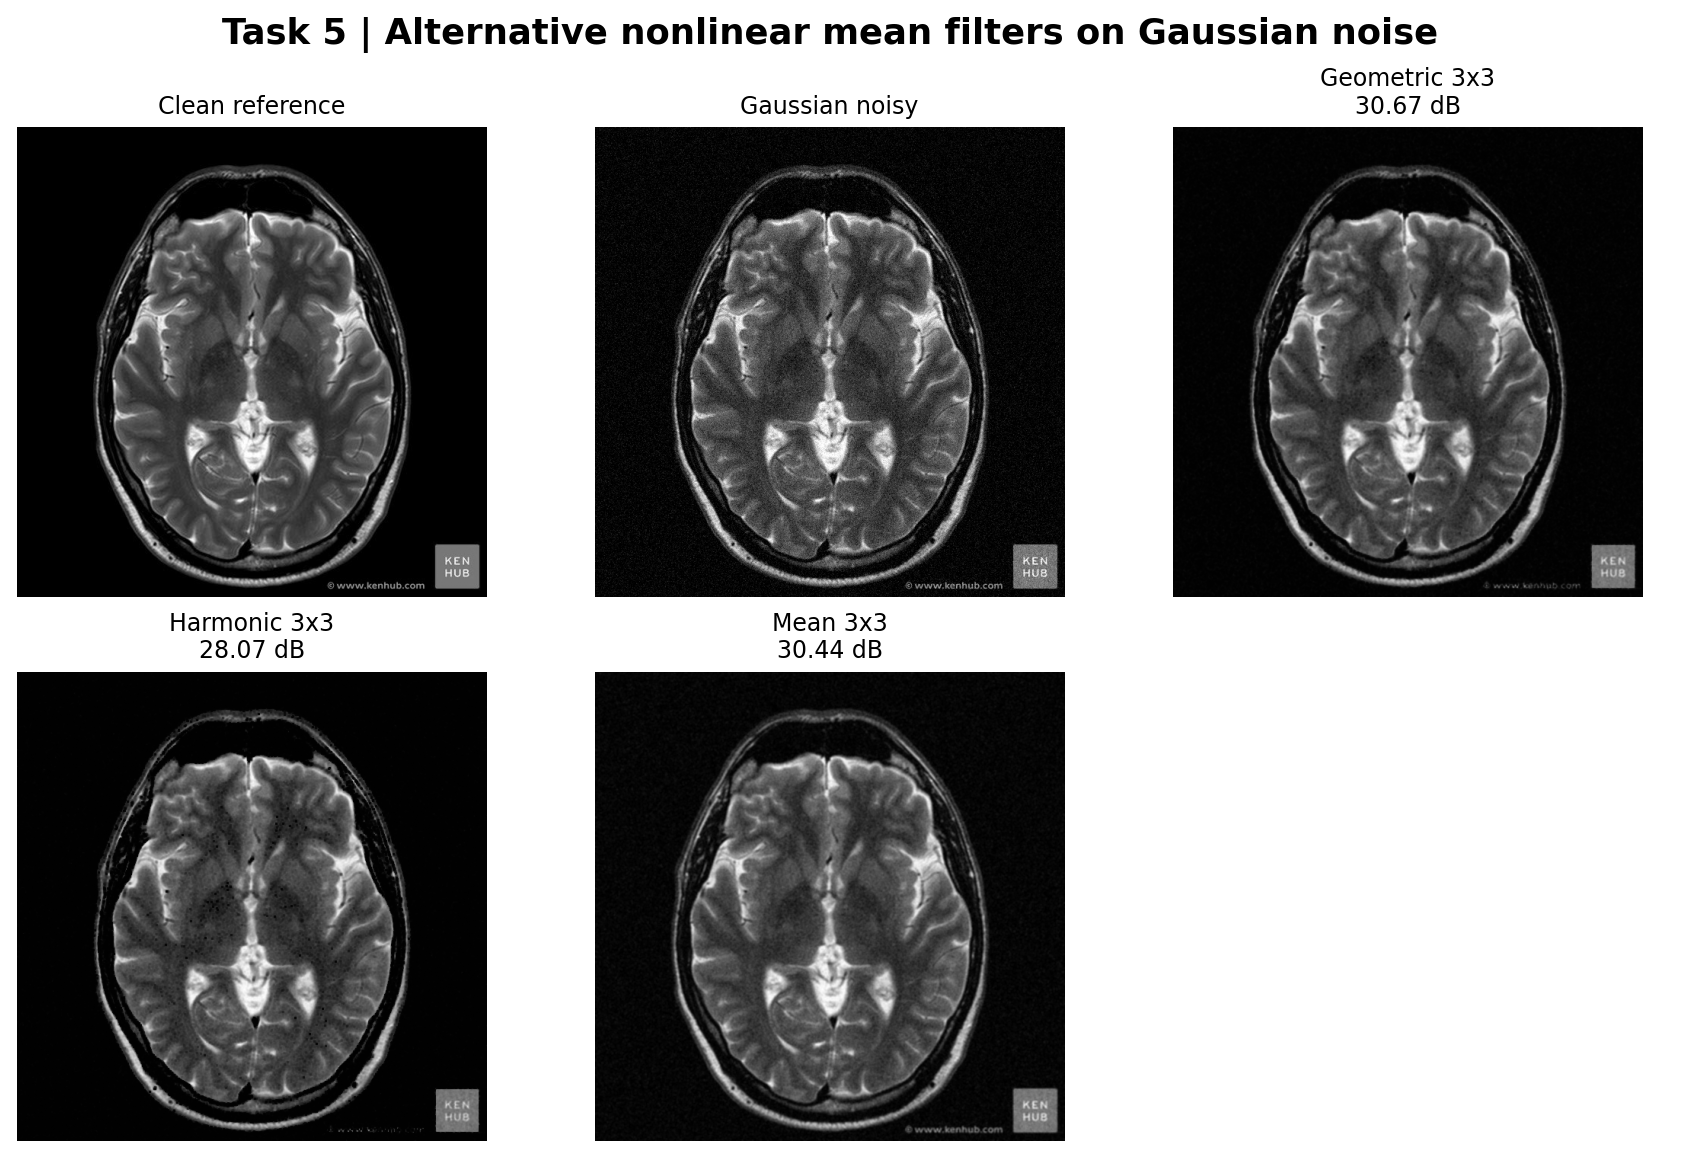
\includegraphics[width=\linewidth,height=0.72\textheight,keepaspectratio]{Figures/F06_mean_variants.png}
\caption{Geometric, harmonic, and arithmetic mean methods for the Gaussian-contaminated image.}
\end{figure}
\begin{figure}[!htbp]
\centering
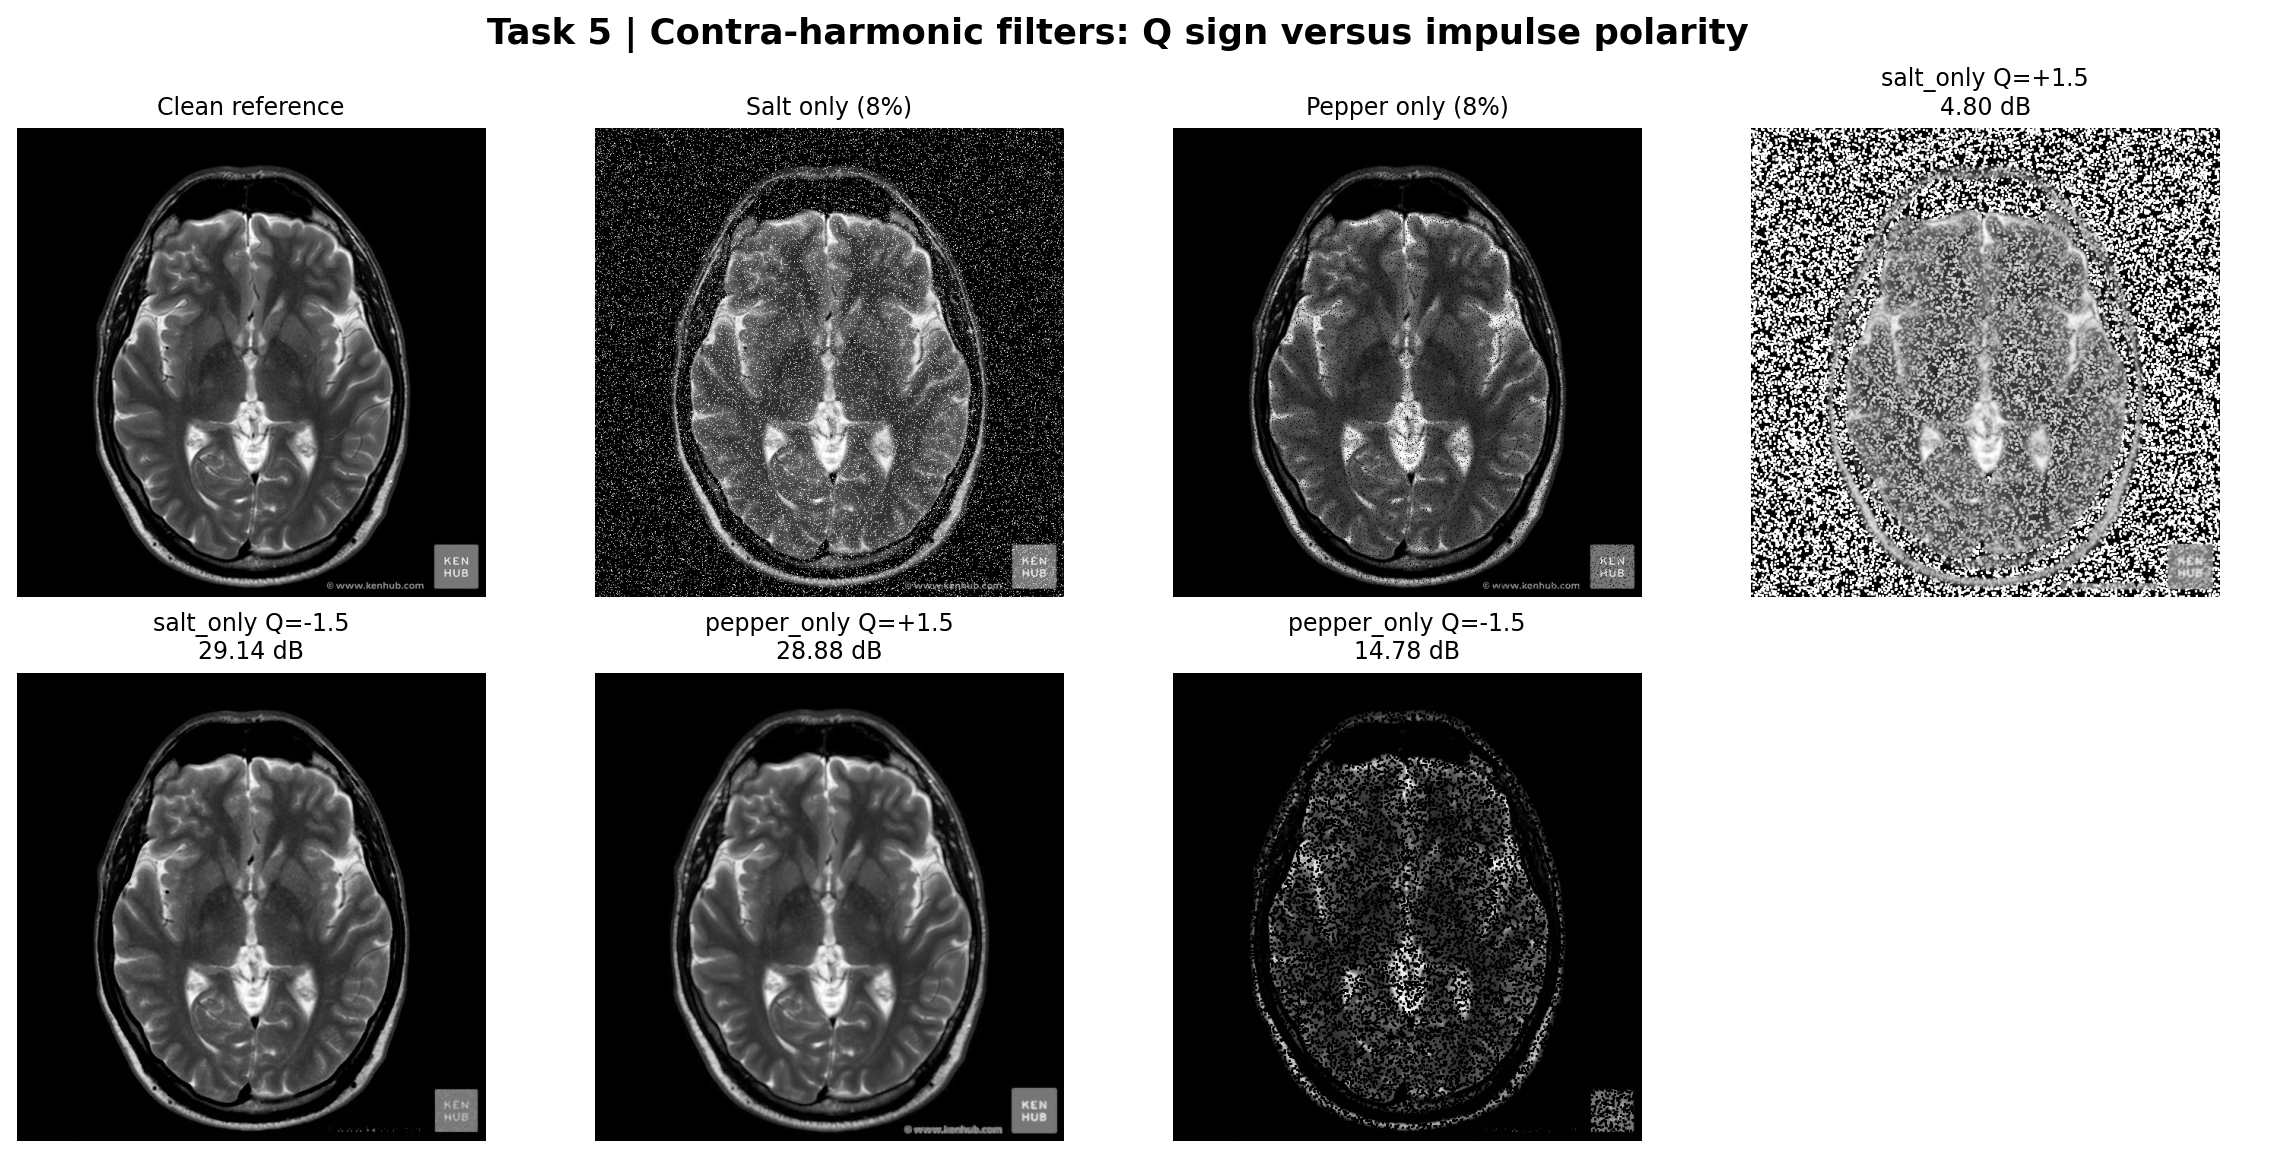
\includegraphics[width=\linewidth,height=0.72\textheight,keepaspectratio]{Figures/F07_contraharmonic.png}
\caption{Opposite Q values tested separately on 8\% salt and 8\% pepper corruption.}
\end{figure}
\begin{longtable}{|p{50.0mm}|p{50.0mm}|p{50.0mm}|}
\caption{Nonlinear filtering and impulse-polarity experiments}\\
\hline
\textbf{Noise case} & \textbf{Method} & \textbf{PSNR (dB)}\\ \hline
\endfirsthead
\hline
\textbf{Noise case} & \textbf{Method} & \textbf{PSNR (dB)}\\ \hline
\endhead
mixed\_salt\_pepper & Noisy & 14.87\\ \hline
mixed\_salt\_pepper & Mean 3x3 & 23.03\\ \hline
mixed\_salt\_pepper & Median 3x3 & 34.88\\ \hline
mixed\_salt\_pepper & Median 5x5 & 30.82\\ \hline
gaussian & Geometric 3x3 & 30.67\\ \hline
gaussian & Harmonic 3x3 & 28.07\\ \hline
gaussian & Mean 3x3 & 30.44\\ \hline
salt\_only & Noisy & 12.14\\ \hline
pepper\_only & Noisy & 22.93\\ \hline
salt\_only & Contra 3x3 Q=+1.5 & 4.80\\ \hline
salt\_only & Contra 3x3 Q=-1.5 & 29.14\\ \hline
pepper\_only & Contra 3x3 Q=+1.5 & 28.88\\ \hline
pepper\_only & Contra 3x3 Q=-1.5 & 14.78\\ \hline
\end{longtable}
Mixed salt-and-pepper noise is restored most successfully here by median 3 x 3 (34.88 dB), versus median 5 x 5 (30.82 dB) and mean 3 x 3 (23.03 dB). For Gaussian noise, the geometric mean gives 30.67 dB, whereas the harmonic mean gives 28.07 dB; the normal arithmetic mean gives 30.44 dB. Contra-harmonic +1.5 on pepper achieves 28.88 dB, compared with 14.78 dB for the wrong sign. The corresponding salt-only results favor -1.5 (29.14 versus 4.80 dB). The salt-only and pepper-only baselines differ because the MRI has extensive dark-background pixels. This illustrates why experiments must report both the corruption model and the reference distribution.

Recommendation based on these runs: median 3 x 3 for mixed impulse contamination; positive-Q contra-harmonic for pepper-only corruption; negative-Q contra-harmonic for salt-only corruption. Wrong-sign contra-harmonic filters can amplify the outlier type they should reject. More strongly weighted nonlinear methods can also introduce local haloing or intensity bias near abrupt edges.

\section{Task 6 - Unsharp masking}
\[ m(x,y)=f(x,y)-f_{\mathrm{blur}}(x,y),\quad g(x,y)=\operatorname{clip}(f(x,y)+\gamma m(x,y),0,1) \]
A Gaussian 5 x 5 smoothing kernel with sigma 1.2 defines the low-frequency estimate. The residual acts as a high-pass component. Tested gains are 0.5, 1.0, and 2.5. The same untouched MRI is used as the source for all gain settings, rather than repeatedly sharpening an already processed image.

\begin{figure}[!htbp]
\centering
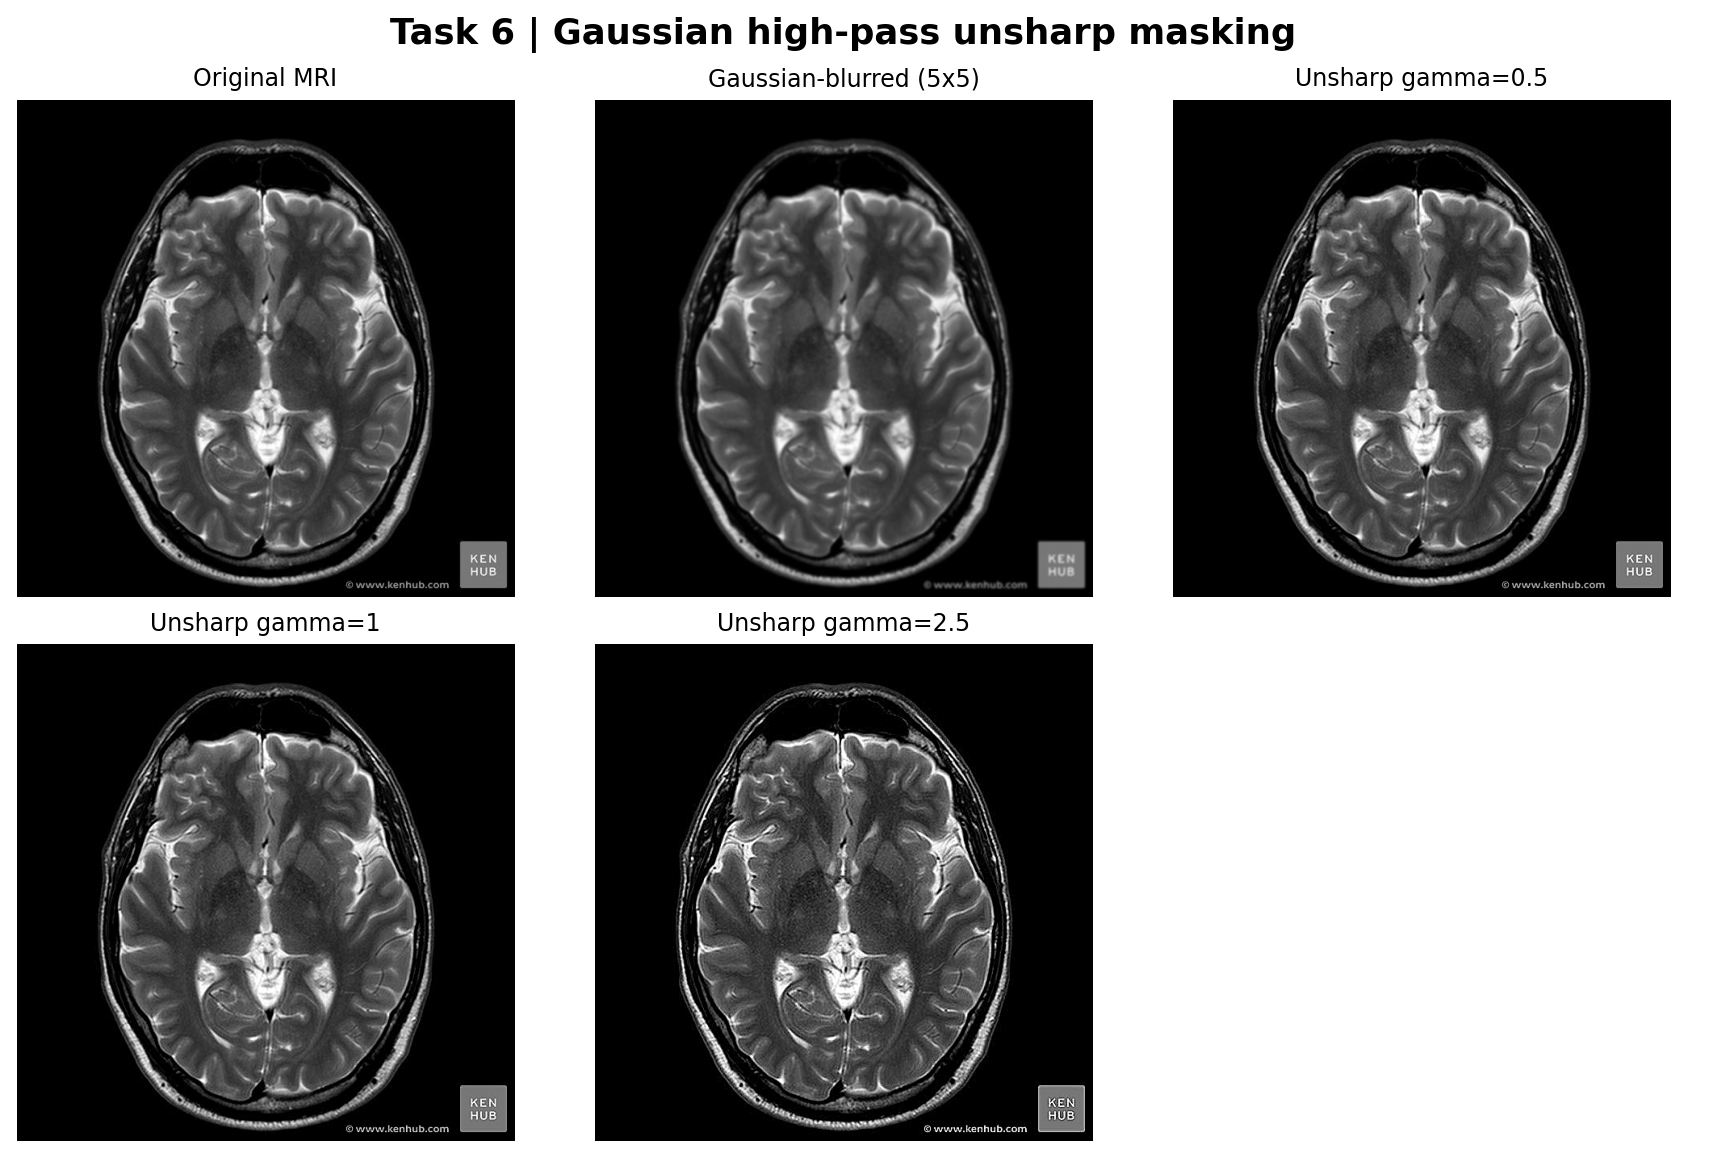
\includegraphics[width=\linewidth,height=0.72\textheight,keepaspectratio]{Figures/F08_unsharp.png}
\caption{Clean input, blurred baseline, and three increasing unsharp gains.}
\end{figure}
\begin{longtable}{|p{50.0mm}|p{50.0mm}|p{50.0mm}|}
\caption{Sharpening gain and clipping behavior}\\
\hline
\textbf{Gain gamma} & \textbf{Pixels requiring clipping (\%)} & \textbf{Mean |change|}\\ \hline
\endfirsthead
\hline
\textbf{Gain gamma} & \textbf{Pixels requiring clipping (\%)} & \textbf{Mean |change|}\\ \hline
\endhead
0.5 & 5.35 & 0.0044\\ \hline
1 & 6.24 & 0.0084\\ \hline
2.5 & 8.01 & 0.0196\\ \hline
\end{longtable}
The fraction of pixels exceeding the valid range before clipping rises from 5.35\% at gamma 0.5 to 8.01\% at gamma 2.5. Gamma 1.0 is a restrained compromise: fine MRI boundaries become more conspicuous without the strongest halos and bright/dark ringing seen at high gain. Clipping counts include the large, nearly black exterior region and should not be interpreted as a clinical quality score. Conventional direct high-frequency enhancement (e.g., adding a Laplacian-derived high-pass response) is closely related, but its derivative kernel and frequency response need not match Gaussian-based unsharp masking.

\section{Task 7 - Sobel, Laplacian, LoG, and DoG}
Sobel computes a pair of first derivatives and combines them as gradient magnitude. It highlights the strength of local intensity transitions and approximately encodes edge orientation. A four-neighbor Laplacian, [0 1 0; 1 -4 1; 0 1 0], is a signed second derivative; edges are commonly associated with its zero crossings, so displaying the absolute response is a visualization of edge-related activity, not a binary edge map. The LoG experiment applies Gaussian smoothing (7 x 7, sigma 1.2) before this Laplacian. DoG subtracts Gaussian smoothings at scales sigma=(1,2) and sigma=(2,4).

\begin{figure}[!htbp]
\centering
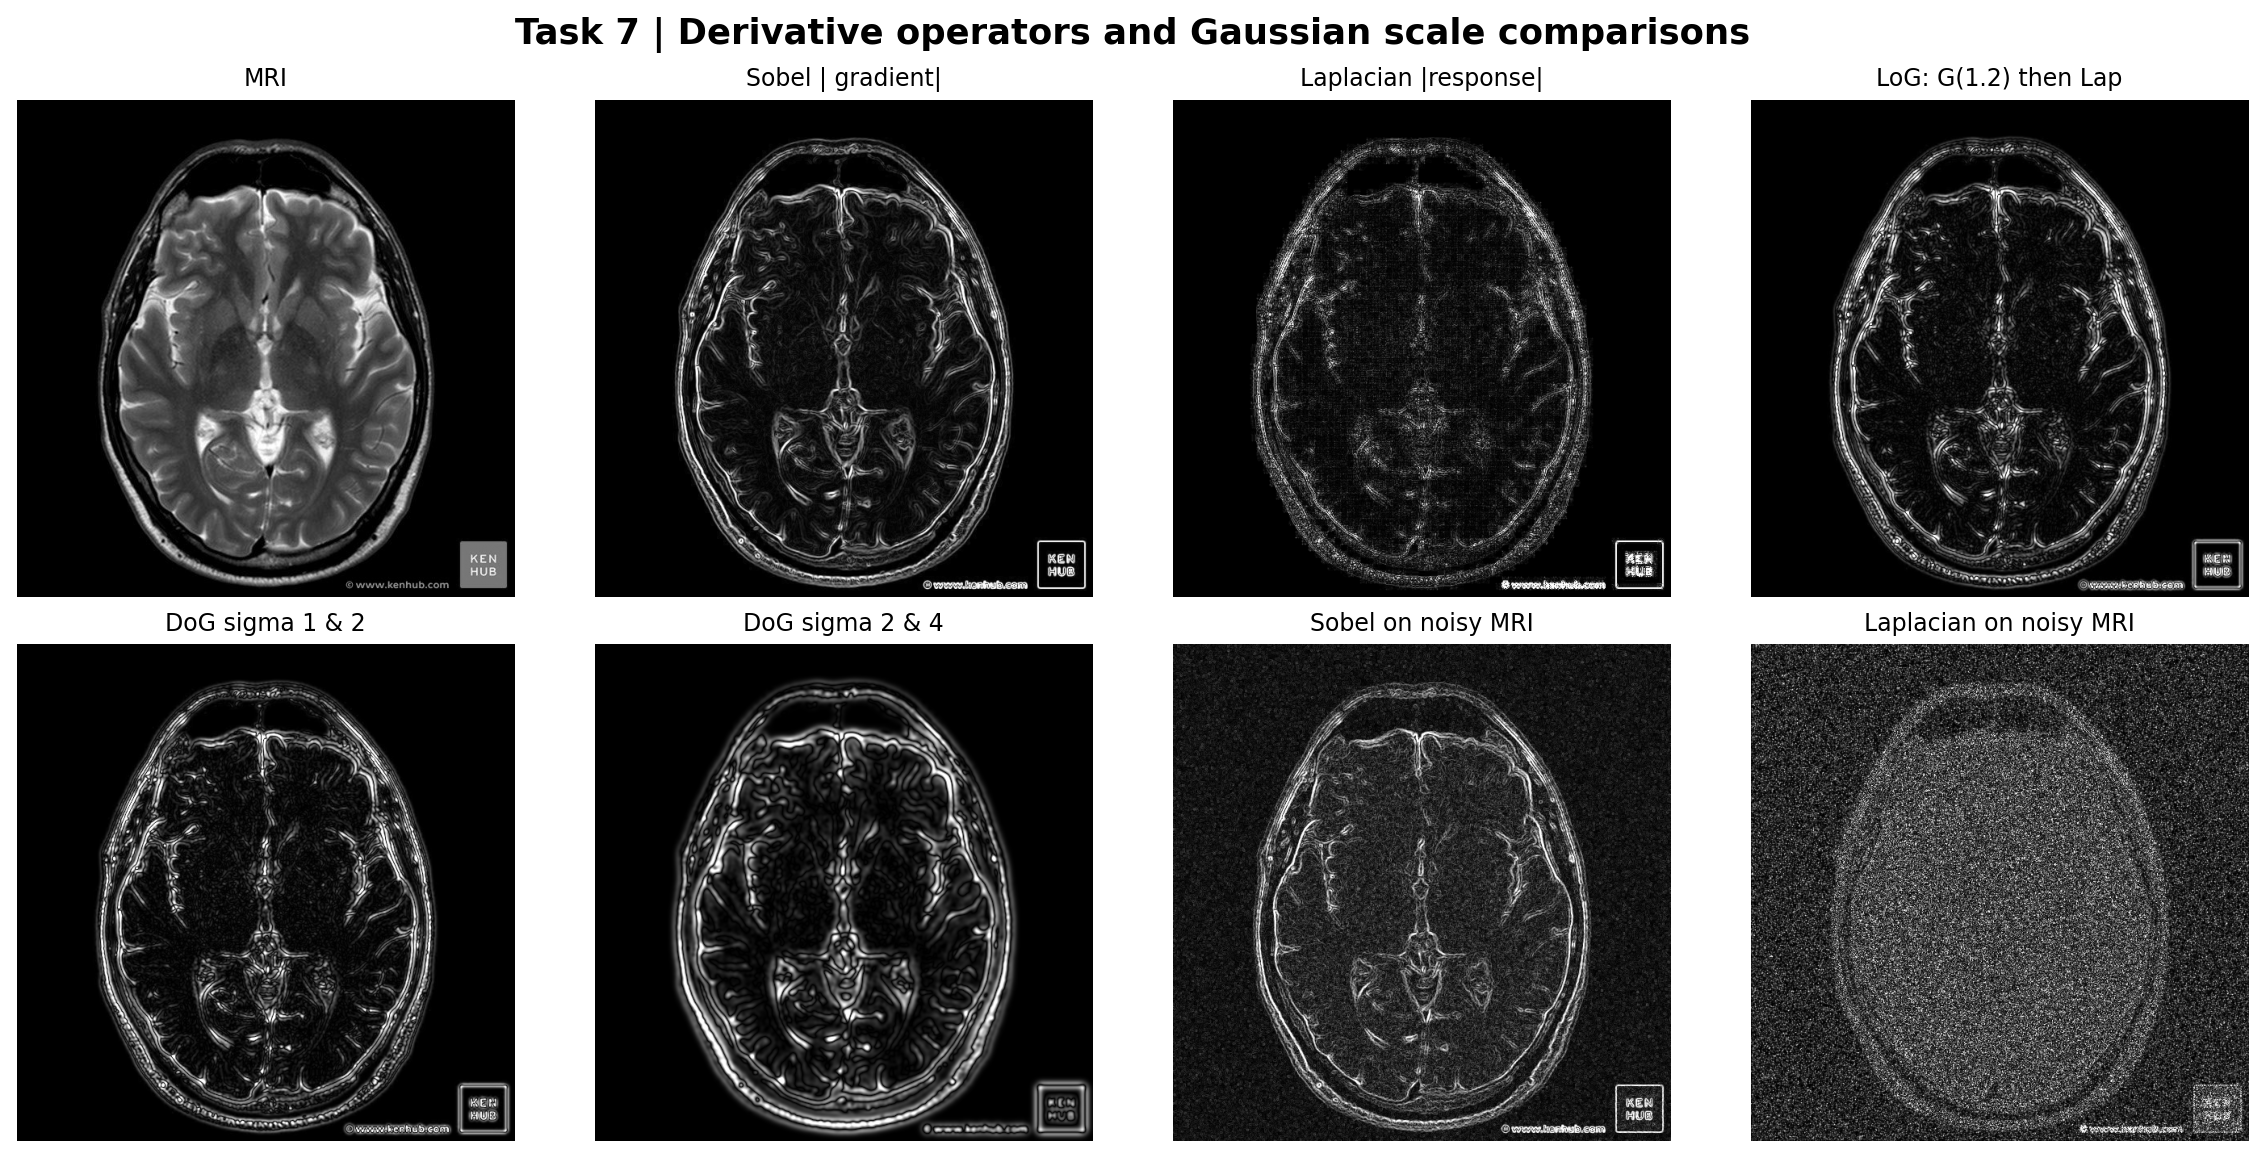
\includegraphics[width=\linewidth,height=0.72\textheight,keepaspectratio]{Figures/F09_edges.png}
\caption{Response magnitudes from Sobel, Laplacian, LoG, and two DoG scales; last two panels illustrate noise sensitivity. Each response is individually normalized to its 99.5th percentile for display.}
\end{figure}
\begin{longtable}{|p{50.0mm}|p{50.0mm}|p{50.0mm}|}
\caption{Derivative response sensitivity to added Gaussian noise}\\
\hline
\textbf{Measure} & \textbf{Clean MRI} & \textbf{Noisy MRI}\\ \hline
\endfirsthead
\hline
\textbf{Measure} & \textbf{Clean MRI} & \textbf{Noisy MRI}\\ \hline
\endhead
Mean Sobel magnitude & 0.0197 & 0.0359\\ \hline
Mean absolute Laplacian & 0.0245 & 0.1657\\ \hline
\end{longtable}
On the clean MRI, Sobel highlights the external head boundary, inner ventricles, and high-gradient tissue interfaces with readable continuity. The unsmoothed Laplacian also responds to very fine intensity changes and becomes conspicuously grainy after noise is added: mean absolute Laplacian response increases from 0.0245 to 0.1657. Sobel mean magnitude increases from 0.0197 to 0.0359. LoG reduces fine-scale noise by suppressing high frequencies before differentiation. DoG approximates a scale-normalized LoG response for nearby scales (up to a sign and scale factor), while the wider (2,4) pair emphasizes broader structures and removes small details. Sobel is the most straightforward choice here for a readable structural-edge preview; LoG is useful for smoothed second-order response analysis [1, 4]. These outputs are illustrative rather than validated anatomical segmentations.

\section{Task 8 - Integrated image processing pipeline}
The test input starts from the same low-contrast chest image used in Task 1. To simulate a difficult acquisition, independent Gaussian noise with sigma 0.03 is added and 2.5\% of pixels are then replaced by an equal mixture of black and white impulses. The complete sequence is (1) median 3 x 3 to remove extreme local outliers before contrast scaling, (2) CLAHE with 8 x 8 tiles and clip limit 0.01 to enhance local contrast, (3) unsharp masking using Gaussian 5 x 5 sigma 1.1 and gamma 0.7 to recover edge crispness. The order matters: enhancing local contrast before removal of impulses would exaggerate contaminated pixels.

\begin{figure}[!htbp]
\centering
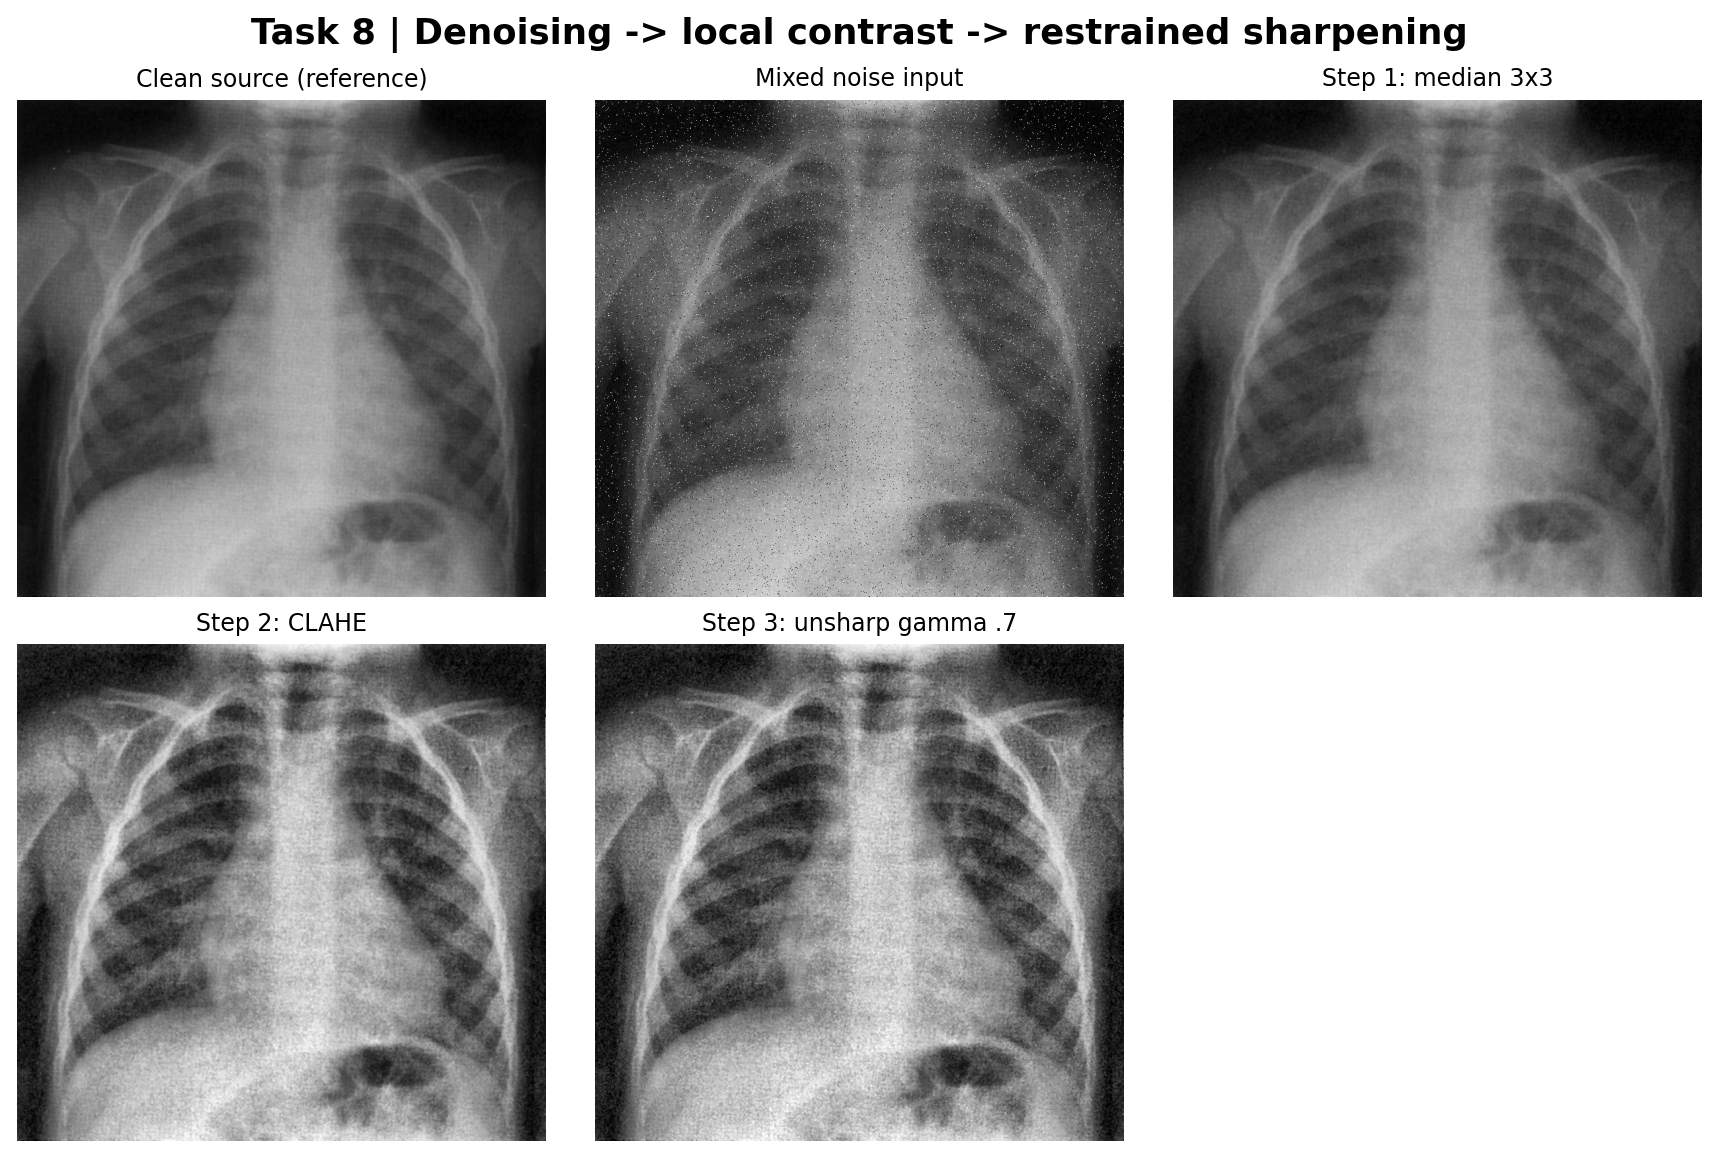
\includegraphics[width=\linewidth,height=0.72\textheight,keepaspectratio]{Figures/F10_pipeline.png}
\caption{Input and every intermediate processing stage, ending with denoise/CLAHE/unsharp result.}
\end{figure}
\begin{longtable}{|p{37.5mm}|p{37.5mm}|p{37.5mm}|p{37.5mm}|}
\caption{End-to-end pipeline stage metrics}\\
\hline
\textbf{Stage} & \textbf{PSNR to clean (dB)} & \textbf{Image std} & \textbf{Entropy (bits)}\\ \hline
\endfirsthead
\hline
\textbf{Stage} & \textbf{PSNR to clean (dB)} & \textbf{Image std} & \textbf{Entropy (bits)}\\ \hline
\endhead
Clean & Reference & 0.1908 & 7.450\\ \hline
Noisy & 20.78 & 0.2069 & 7.514\\ \hline
Median & 37.20 & 0.1909 & 7.470\\ \hline
CLAHE & 17.64 & 0.2244 & 7.778\\ \hline
Final & 17.39 & 0.2269 & 7.808\\ \hline
\end{longtable}
The noisy image starts at 20.78 dB. Median filtering removes many impulses and improves reference fidelity to 37.20 dB. CLAHE changes intended local brightness mapping, reducing PSNR to 17.64 dB while raising global gray-level standard deviation from 0.191 to 0.224; the final unsharp stage increases it slightly to 0.227. Entropy increases from 7.470 bits after denoising to 7.808 bits in the final result. The final stage has PSNR 17.39 dB, lower than the original noisy input; this is expected when deliberate tone remapping is penalized against an untouched reference. It does not by itself invalidate contrast enhancement.

The final image displays clearer rib/lung boundaries in the radiograph illustration, but some fine grain and local intensity distortions remain. Limitations: a median filter may erase thin line structures; CLAHE can still amplify residual noise; unsharp masking may produce overshoot and ringing; no expert reference annotation is available. An alternate CLAHE -> median -> unsharp sequence may first amplify isolated impulses and then suppress some of the enhanced details; it should be re-evaluated rather than assumed to be superior. A conservative alternative for primarily Gaussian noise is Gaussian smoothing -> CLAHE -> restrained unsharp masking.

\section{Cross-task findings and limitations}
The manual spatial operation shows that kernel orientation changes the sign for a directional, asymmetric filter. The separable Gaussian saves one-third of interior multiplications for the 3 x 3 case without materially changing the output. Gaussian noise responds well to small Gaussian smoothing, while sparse impulsive contamination is addressed more effectively by a 3 x 3 median filter. Contra-harmonic filtering depends crucially on the polarity of impulse noise, the Q sign, and the handling of zero-valued pixels. Edge operators are sensitive to both the differential order and image noise; scale selection and preprocessing are as important as the specific operator name. Finally, boosting contrast is a perceptual transformation and need not improve PSNR against the unenhanced image.

Challenges and possible sources of disagreement include: differences between MATLAB adapthisteq and scikit-image CLAHE histogram clipping/interpolation; alternate definitions of reflect versus mirror at the edge; finite numerical precision; image watermarks or non-anatomical text; the use of fixed 8-bit noise samples; gamma/contrast changes that reduce direct PSNR; and the absence of clinical ground truth. These limitations are explicitly documented to prevent the numerical results from being overinterpreted.

\section{Reproduction instructions, image sources, and deliverables}
Source files: Source\_Images/Original\_Samples/image3.jpg (chest radiograph) and image2.jpg (MRI) are included unchanged from the instructor-provided Image Samples folder; the other instructor-provided media, including two DICOM files, are preserved unmodified for completeness but are not analyzed. Grayscale derivatives and noisy images are in Source\_Images/Prepared\_Inputs. No externally sourced medical images or hidden datasets were used [7].

Reproducibility materials are organized separately from the report in the repository. The MATLAB implementation is located in MATLAB/run\_assignment2.m (requires Image Processing Toolbox); the executed Python reference is in Python\_Reference/reproduce\_results.py. Original and fixed prepared inputs are retained under Source\_Images, and machine-readable metrics are in Outputs/Results. The repository README documents installation, execution, validation, and the distinction between MATLAB and Python outputs; see the MATLAB Image Processing Toolbox references for relevant MATLAB operator definitions [5, 6].

The Report folder contains the present report in Word and PDF, an Overleaf-compatible main.tex, and its 11 figure files. No source code is reproduced within the report, including its appendices; complete implementation files are available only in the repository source directories. The original assignment instructions are included separately for reference. This arrangement preserves the report as a results-and-discussion document while allowing independent inspection of the implementation.

\section{GitHub repository and source files}
The complete implementation and reproducibility materials are maintained separately from this report in the associated GitHub repository. The repository includes the MATLAB implementation, the executed Python reference, prepared image inputs, measurement tables, figures, and validation checks. No source-code listings are included in this document.

\noindent\url{https://github.com/burakcakirer/ee3005-image-processing-assignment-2}

Repository publication note: The link above is the intended GitHub address and will work after the project is published under the specified username and repository name. If the published repository is renamed, update this link in all report formats before submission.

\clearpage
\section{References}
\noindent\hangindent=1.5em\hangafter=1 [1] R. C. Gonzalez and R. E. Woods, Digital Image Processing, 4th ed. Pearson, 2018.\par

\noindent\hangindent=1.5em\hangafter=1 [2] K. Zuiderveld, "Contrast Limited Adaptive Histogram Equalization," in Graphics Gems IV, P. S. Heckbert, Ed. Academic Press, 1994, pp. 474-485.\par

\noindent\hangindent=1.5em\hangafter=1 [3] W. K. Pratt, Digital Image Processing, 4th ed. Wiley-Interscience, 2007.\par

\noindent\hangindent=1.5em\hangafter=1 [4] D. Marr and E. Hildreth, "Theory of edge detection," Proceedings of the Royal Society of London. Series B, Biological Sciences, vol. 207, no. 1167, pp. 187-217, 1980. DOI: 10.1098/rspb.1980.0020.\par

\noindent\hangindent=1.5em\hangafter=1 [5] MathWorks, "adapthisteq: Contrast-limited adaptive histogram equalization (CLAHE)," Image Processing Toolbox Documentation. https://www.mathworks.com/help/images/ref/adapthisteq.html (accessed 20 October 2026).\par

\noindent\hangindent=1.5em\hangafter=1 [6] MathWorks, "imfilter: N-D filtering of multidimensional images," Image Processing Toolbox Documentation. https://www.mathworks.com/help/images/ref/imfilter.html (accessed 20 October 2026).\par

\noindent\hangindent=1.5em\hangafter=1 [7] Course-provided Image Processing Assignment 2 instructions and accompanying image samples, EE3005 Biomedical System Design Capsule-S1, Abdullah Gul University, 2026. Unpublished course materials.\par

\end{document}
